% $Header: /cvsroot/latex-beamer/latex-beamer/solutions/conference-talks/conference-ornate-20min.en.tex,v 1.6 2004/10/07 20:53:08 tantau Exp $

\documentclass{beamer}

% This file is a solution template for:

% - Talk at a conference/colloquium.
% - Talk length is about 20min.
% - Style is ornate.



% Copyright 2004 by Till Tantau <tantau@users.sourceforge.net>.
%
% In principle, this file can be redistributed and/or modified under
% the terms of the GNU Public License, version 2.
%
% However, this file is supposed to be a template to be modified
% for your own needs. For this reason, if you use this file as a
% template and not specifically distribute it as part of a another
% package/program, I grant the extra permission to freely copy and
% modify this file as you see fit and even to delete this copyright
% notice.


\mode<presentation>
{
%  \usetheme{Warsaw}
%  \usetheme{Boadilla}
%  \usetheme{Goettingen}
%  \usetheme{Hannover}
%  \usetheme{Madrid}
%  \usetheme{Marburg}
%  \usetheme{Montpellier}
%  \usetheme{Pittsburgh}
  \usetheme{Hawke}
  % or ...

  \setbeamercovered{transparent}
  % or whatever (possibly just delete it)
}


\usepackage[english]{babel}
% or whatever

\usepackage[latin1]{inputenc}
% or whatever

\usepackage{times}
\usepackage[T1]{fontenc}
% Or whatever. Note that the encoding and the font should match. If T1
% does not look nice, try deleting the line with the fontenc.

\usepackage{multimedia}


%%%%%%
% My Commands
%%%%%%

\newcommand{\ml}{{\sc matlab}}

%%%%

\title[Lecture 6] % (optional, use only with long paper titles)
{Lecture 6 - Nonlinear equations and bisection}

% \subtitle
% {Include Only If Paper Has a Subtitle}

\author[I. Hawke] % (optional, use only with lots of authors)
{I.~Hawke}
% - Give the names in the same order as the appear in the paper.
% - Use the \inst{?} command only if the authors have different
%   affiliation.

\institute[University of Southampton] % (optional, but mostly needed)
{
%  \inst{1}%
  School of Mathematics, \\
  University of Southampton, UK
}
% - Use the \inst command only if there are several affiliations.
% - Keep it simple, no one is interested in your street address.

\date[Semester 1] % (optional, should be abbreviation of conference name)
{MATH3018/6141, Semester 1}
% - Either use conference name or its abbreviation.
% - Not really informative to the audience, more for people (including
%   yourself) who are reading the slides online

\subject{Numerical methods}
% This is only inserted into the PDF information catalog. Can be left
% out.



% If you have a file called "university-logo-filename.xxx", where xxx
% is a graphic format that can be processed by latex or pdflatex,
% resp., then you can add a logo as follows:

\pgfdeclareimage[height=0.5cm]{university-logo}{mathematics_7469}
\logo{\pgfuseimage{university-logo}}



% Delete this, if you do not want the table of contents to pop up at
% the beginning of each subsection:
%  \AtBeginSubsection[]
%  {
%    \begin{frame}<beamer>
%      \frametitle{Outline}
%      \tableofcontents[currentsection,currentsubsection]
%    \end{frame}
%  }
\AtBeginSection[]
{
  \begin{frame}<beamer>
    \frametitle{Outline}
    \tableofcontents[currentsection]
  \end{frame}
}


% If you wish to uncover everything in a step-wise fashion, uncomment
% the following command:

%\beamerdefaultoverlayspecification{<+->}


\begin{document}

\begin{frame}
  \titlepage
\end{frame}

\section{Nonlinear equations}

\subsection{Nonlinear equations}

\begin{frame}
  \frametitle{Nonlinear equations}

  A large number of nonlinear equations obviously \emph{have}
  solutions, but the solutions cannot always be found in closed form.

  \begin{center}
    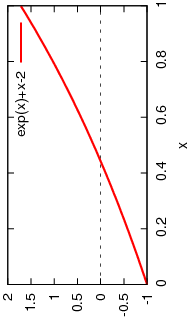
\includegraphics[angle=-90,width=0.65\textwidth]{figures/Nonlinear1}
  \end{center} \pause

  Numerical methods %for the solution of nonlinear equations
  can give accurate, approximate solutions.% to these sort of equations.

  % As always the methods used in practice are based on the ideas
  % presented but are much, much more complicated.

\end{frame}

\begin{frame}
  \frametitle{Framework}

%  The nonlinear equations we will look at can always be written as
  Write the problem as
  %
  \begin{equation*}
    f(x) = 0.
  \end{equation*}
  %
  Goal: given $f$, find $x$. \pause

  \vspace{1ex}

  Assume: $f$ real, continuous. Sometimes restrict to $f$ differentiable. \pause

  % We are trying to find $x$ to satisfy this equation, given
  % $f$. \pause We always assume $f$ is real; we have to assume $f$ is
  % continuous; we may assume $f$ is differentiable. \pause

  \vspace{1ex}

%  In some cases we
  May consider equivalent problem
  \begin{equation*}
    g(x) = x.
  \end{equation*}
  %
  % Clearly setting $g(x) = f(x) + x$ gives the same problem. \pause
  % This has a different geometric interpretation, as we will see
  % later. \pause
  Same problem, different (geometric) interpretation. \pause

  \vspace{1ex}

  % In all cases we
  Assume that evaluating $f$ or $g$ is \emph{expensive}. Want to minimize the number of evaluations.

\end{frame}

\begin{frame}
  \frametitle{Bisection method}

  Given $f: x \in \mathbb{R} \to \mathbb{R}$, continuous, find $x$ such that
  \begin{equation*}
    f(x) = 0.
  \end{equation*}

  \vspace{2ex}

  \begin{columns}
    \begin{column}{0.5\textwidth}
      Simple and robust method: \emph{bisection}. Assume we have found (somehow!) two points, $x^{(L)}$ and $x^{(R)}$ that bracket root. \pause

      \vspace{0.5ex}

      Check halfway point $x^{(M)}$. Either $f(x^{(M)})=0$ (problem solved), or $x^{(M)}$ and one of $x^{(L,R)}$ bracket the root. \pause

      \vspace{0.5ex}

      Repeat to converge.
    \end{column}
    \begin{column}{0.475\textwidth}
      \begin{overlayarea}{\textwidth}{0.5\textheight}
        \only<1|handout:0>
        {
          \begin{center}
            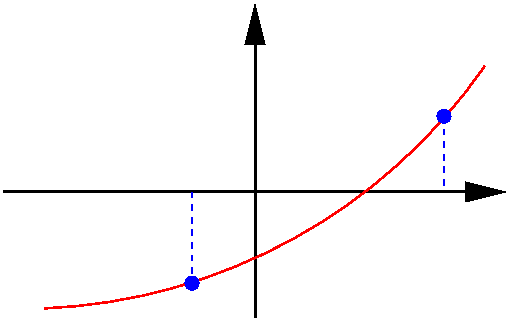
\includegraphics[width=\textwidth]{figures/Bisection1}
          \end{center}
        }
        \only<2|handout:0> {
          \begin{center}
            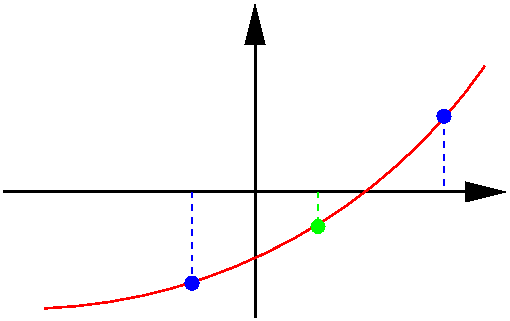
\includegraphics[width=\textwidth]{figures/Bisection2}
          \end{center}
        }
        \only<3|handout:1> {
          \begin{center}
            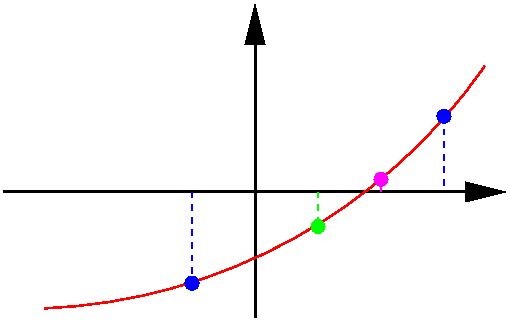
\includegraphics[width=\textwidth]{figures/Bisection3}
          \end{center}
        }
      \end{overlayarea}
    \end{column}
  \end{columns}

\end{frame}

\begin{frame}
  \frametitle{Starting}

  To start need at least one root in $[x^{(L)}, x^{(R)}]$. Can compute $f(x^{(L)})$, $f(x^{(R)})$. \pause

  \begin{columns}
    \begin{column}{0.5\textwidth}
      Simple test
        $f(x^{(L)}) \times f(x^{(R)}) < 0$
      works for odd number of roots. \pause

      \vspace{0.5ex}

      Cannot distinguish even number of roots and no
      roots. \pause Doubling size of interval
      may work; otherwise human intervention best.
    \end{column}
    \begin{column}{0.5\textwidth}
      \includegraphics<2|handout:0>[width=\textwidth]{figures/BisectionStart1}
      \includegraphics<3|handout:1>[width=\textwidth]{figures/BisectionStart2}
      \includegraphics<4|handout:2>[width=\textwidth]{figures/BisectionStart3}
    \end{column}
  \end{columns}

\end{frame}

\begin{frame}
  \frametitle{Stopping}

  When is the answer ``accurate enough''? \pause Two obvious
  stopping criteria:

  \vspace{2ex}

  \begin{columns}
    \begin{column}{0.5\textwidth}
      \begin{overlayarea}{\textwidth}{0.6\textheight}
        \only<2|handout:1>
        {
          \begin{enumerate}
          \item $|f(x_n^{(M)})| < \epsilon$.
          \end{enumerate}

          \vspace{2ex}

          This fails in the case on the right.
        }
        \only<3|handout:0>
        {
          \begin{enumerate}
          \item $|f(x_n^{(M)})| < \epsilon$.
          \item $|x_n^{(R)} - x_n^{(L)}| < \delta$.
          \end{enumerate}


          \vspace{2ex}

          This fails in the case on the right.
        }
        \only<4|handout:2>
        {
          \begin{enumerate}
          \item $|f(x_n^{(M)})| < \epsilon$.
          \item $|x_n^{(R)} - x_n^{(L)}| < \delta$.
          \end{enumerate}


          \vspace{2ex}

          This fails in the case on the right.

          \vspace{2ex}

          Use both, and restrict number of iterations.
        }
      \end{overlayarea}
    \end{column}
    \begin{column}{0.475\textwidth}
      \begin{overlayarea}{\textwidth}{0.6\textheight}
        \only<2|handout:1>
        {
          \begin{center}
            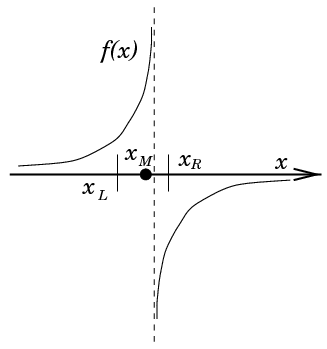
\includegraphics[width=0.9\textwidth]{figures/bisec_stop_1}
          \end{center}
        }
        \only<3-|handout:2>
        {
          \begin{center}
            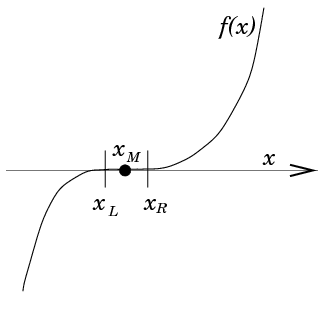
\includegraphics[width=0.9\textwidth]{figures/bisec_stop_2}
          \end{center}
        }
      \end{overlayarea}
    \end{column}
  \end{columns}

\end{frame}

\begin{frame}
  \frametitle{Example}

  Apply bisection to
  \begin{equation*}
    f(x) = e^x + x - 2 = 0
  \end{equation*}
  on the domain $x \in [0,1]$. \pause

  \vspace{2ex}

  \begin{columns}
    \begin{column}{0.5\textwidth}
      Start: interval is entire domain;
      function values show an odd number of roots.\pause

      \vspace{0.5ex}

      Two steps: 25\% of interval.\pause

      \vspace{0.5ex}

      Five steps: 3\% of interval.\pause

      \vspace{0.5ex}

      Ten steps: root is ``found''.\pause

      \vspace{0.5ex}

      33 steps: function is zero to $10^{-10}$.
    \end{column}
    \begin{column}{0.5\textwidth}
      \includegraphics<2|handout:0>[width=\textwidth]{figures/BisectionExample1}
      \includegraphics<3|handout:0>[width=\textwidth]{figures/BisectionExample2}
      \includegraphics<4|handout:0>[width=\textwidth]{figures/BisectionExample3}
      \includegraphics<5-|handout:1>[width=\textwidth]{figures/BisectionExample4}
    \end{column}
  \end{columns}

\end{frame}

\begin{frame}
  \frametitle{Bisection convergence}

  \begin{columns}
    \begin{column}{0.5\textwidth}
      Convergence is \emph{linear}: each iteration reduces error by
      constant factor.

      \vspace{1ex}

      Clear as root inside interval; error reduces by constant amount each
      iteration.
    \end{column}
    \begin{column}{0.5\textwidth}
      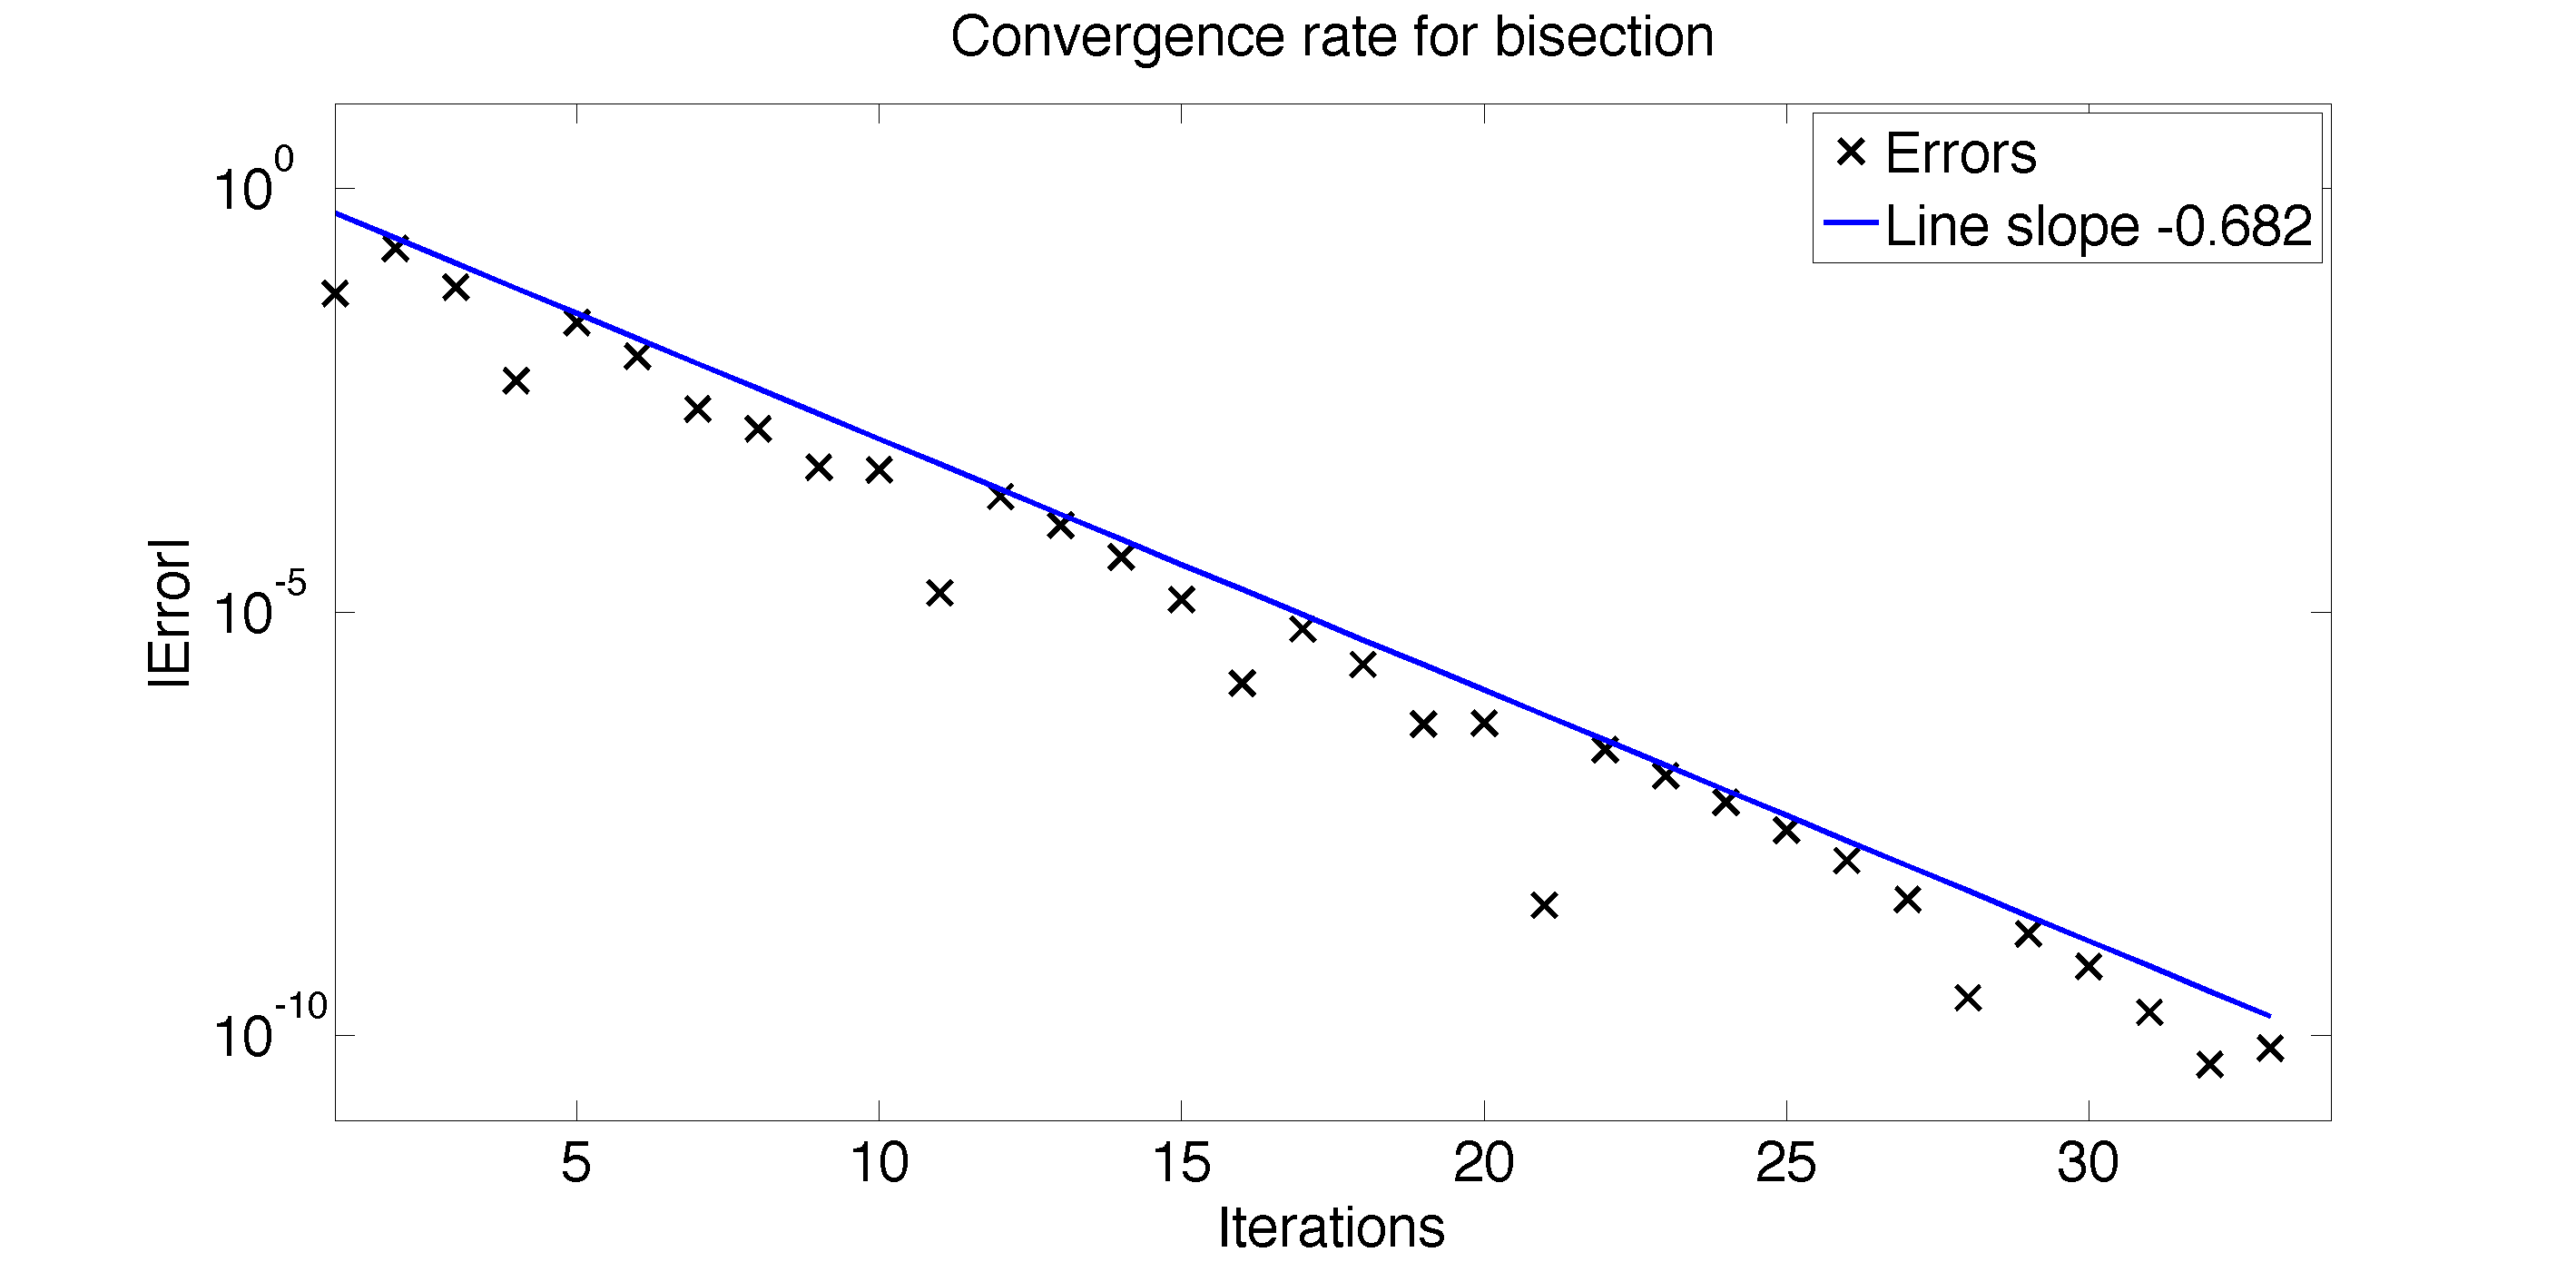
\includegraphics[width=\textwidth]{figures/BisectionConvergence}
    \end{column}
  \end{columns}

\end{frame}

\section{Summary}

\subsection{Summary}

\begin{frame}
  \frametitle{Summary}

  \begin{itemize}
  \item The simplest method for solving nonlinear equations $f(x) = 0$
    is the bisection method:
    \begin{itemize}
    \item Find two points $x^{(L)}$, $x^{(R)}$ such that $f(x^{(L)})
      \, f(x^{(R)}) < 0$.
    \item Find the midpoint $x^{(M)}$. If this is not sufficiently
      accurate, replace either $x^{(L)}$ or $x^{(R)}$ with $x^{(M)}$
      as appropriate so that the root is still bracketed.
    \item Repeat as necessary.
    \end{itemize}
  \item Normally to stop the algorithm any one of the following is sufficient:
    \begin{enumerate}
    \item Too many iterations are performed.
    \item The estimated root $f(x^{(M)})$ is sufficiently small.
    \item The interval is sufficiently small.
    \end{enumerate}
  \item The error in the root location at step $n$ is always less then
    $(x^{(R)}_0 - x^{(L)}_0) / 2^n$.
  \item Bisection always converges, but is slow.
  \item Generalizing to systems is hard; how to bracket root?
  \end{itemize}

\end{frame}

\end{document}



%%% Local Variables:
%%% mode: latex
%%% TeX-master: t
%%% End:
